\chapter{Triển khai hệ thống}

\section{Môi trường triển khai}

Hệ thống ChatBot được triển khai theo mô hình Client--Server. Phần giao diện người dùng được xây dựng bằng ReactJS, Backend sử dụng FastAPI và toàn bộ dữ liệu vector được lưu trên ChromaDB. Hệ thống AI sử dụng mô hình Gemini 2.5 Flash kết hợp với cơ chế Retrieval-Augmented Generation (RAG).

Trong quá trình triển khai, hệ thống được chia thành các module riêng biệt gồm:

\begin{itemize}
	\item Giao diện người dùng (Frontend)
	\item API xử lý nghiệp vụ (FastAPI)
	\item Module RAG
	\item ChromaDB
	\item Module Benchmark
	\item Dashboard thống kê
\end{itemize}

\section{Chức năng Chat Sandbox}

Chat Sandbox là chức năng chính của hệ thống, cho phép sinh viên đặt câu hỏi trực tiếp dựa trên các tài liệu đã được tải lên.

\begin{figure}[H]
	\centering
	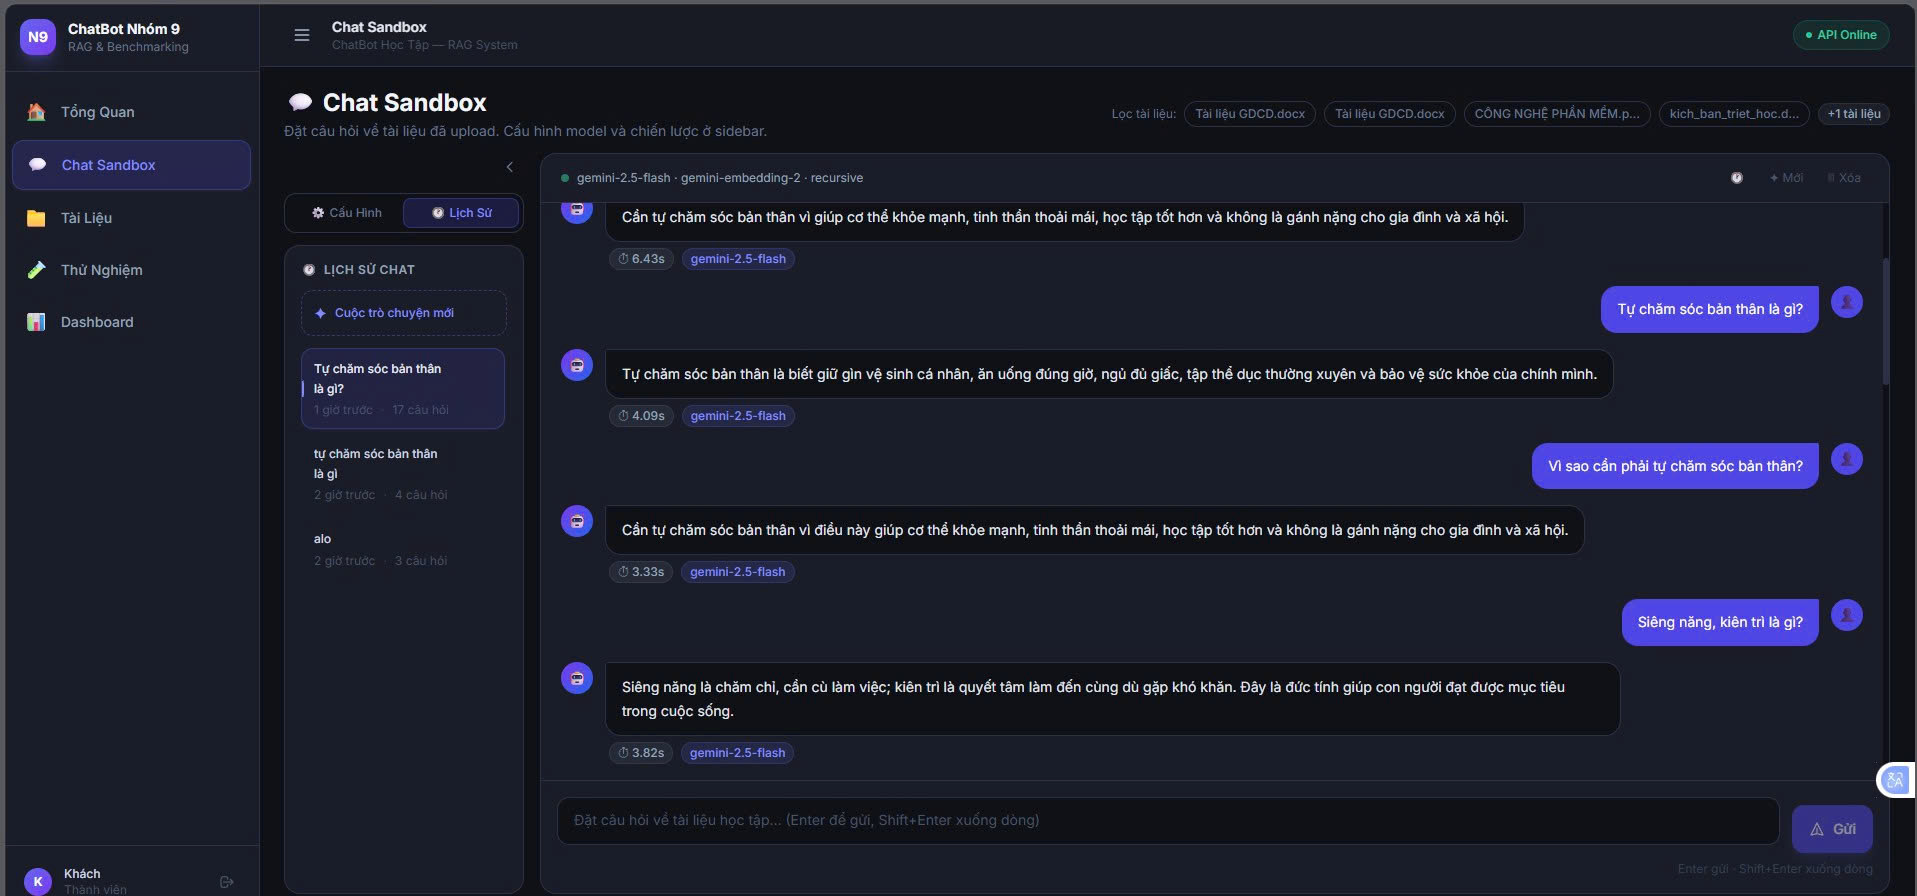
\includegraphics[width=\textwidth]{images/test_1}
	\caption{Giao diện Chat Sandbox}
	\label{fig:chat_sandbox}
\end{figure}
Sau khi người dùng nhập câu hỏi, hệ thống sẽ gửi yêu cầu đến FastAPI.

Backend tiến hành:

\begin{enumerate}
	\item Nhận câu hỏi
	\item Thực hiện embedding
	\item Truy vấn ChromaDB
	\item Lấy các đoạn tài liệu liên quan
	\item Tạo Prompt hoàn chỉnh
	\item Gửi sang Gemini 2.5 Flash
	\item Nhận kết quả
	\item Hiển thị lên giao diện
\end{enumerate}

Ngoài nội dung trả lời, hệ thống còn hiển thị:

\begin{itemize}
	\item Model AI sử dụng
	\item Thời gian phản hồi
	\item Lịch sử hội thoại
	\item Danh sách tài liệu đang được sử dụng
\end{itemize}

Việc lưu lịch sử hội thoại giúp người dùng dễ dàng tiếp tục trao đổi mà không cần nhập lại các câu hỏi trước đó.
\section{Chức năng quản lý tài liệu}

Hệ thống cho phép quản trị viên tải lên các tài liệu PDF hoặc DOCX để xây dựng kho tri thức phục vụ quá trình Retrieval.

\begin{figure}[H]
	\centering
	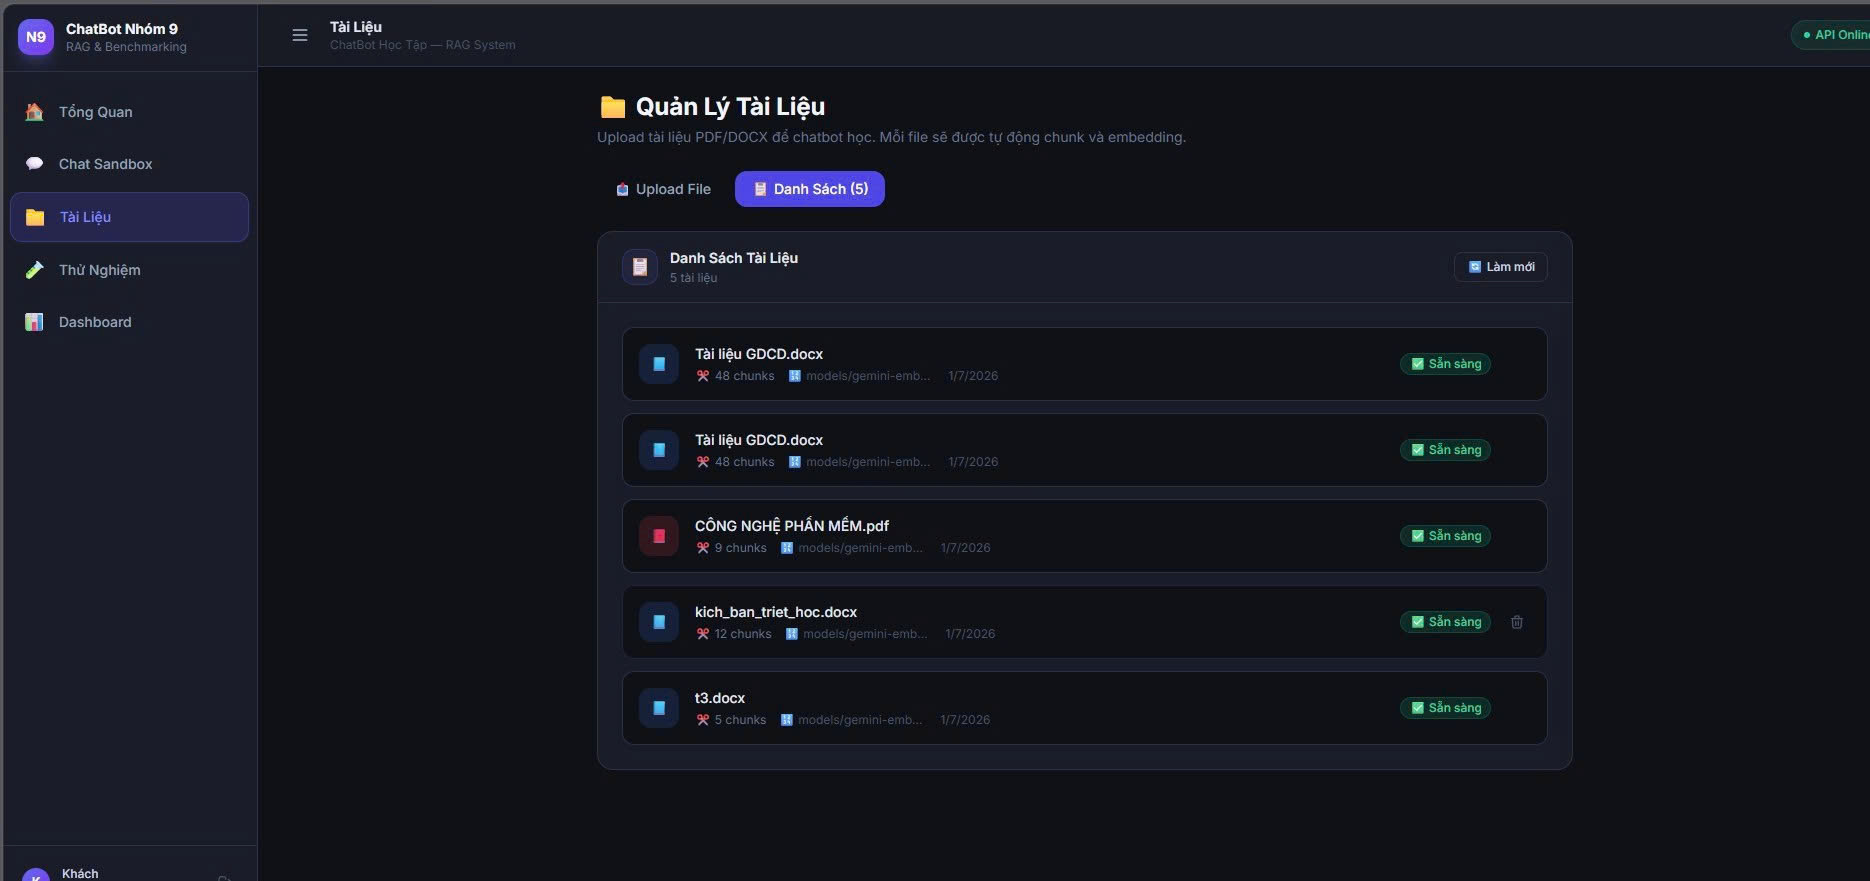
\includegraphics[width=\textwidth]{images/test_2}
	\caption{Chức năng quản lý tài liệu}
	\label{fig:document}
\end{figure}
Sau khi tải lên, hệ thống tự động thực hiện:

\begin{itemize}
	\item Đọc nội dung tài liệu
	\item Chia tài liệu thành nhiều đoạn (Chunking)
	\item Sinh Vector Embedding
	\item Lưu vào ChromaDB
	\item Cập nhật trạng thái tài liệu
\end{itemize}

Danh sách tài liệu sẽ hiển thị:

\begin{itemize}
	\item Tên tài liệu
	\item Số lượng Chunk
	\item Mô hình Embedding
	\item Ngày tải lên
	\item Trạng thái xử lý
\end{itemize}

Khi trạng thái chuyển sang "Sẵn sàng", tài liệu có thể được sử dụng để trả lời câu hỏi trong Chat Sandbox.

\section{Luồng xử lý của hệ thống RAG}

Quá trình xử lý của hệ thống được thực hiện theo các bước:

\begin{enumerate}
	\item Người dùng nhập câu hỏi.
	\item FastAPI nhận request.
	\item Sinh vector embedding cho câu hỏi.
	\item Truy vấn ChromaDB.
	\item Lấy Top-K đoạn tài liệu phù hợp.
	\item Ghép Prompt.
	\item Gửi Prompt sang Gemini.
	\item Gemini sinh câu trả lời.
	\item Hiển thị kết quả lên giao diện.
\end{enumerate}

Quy trình trên giúp hạn chế hiện tượng AI trả lời ngoài phạm vi dữ liệu và nâng cao độ chính xác của câu trả lời.